\newpage
\subsection{Hidden Subset}
\label{Hidden Subset}
Analog zu den \textit{Naked Subset}-Techniken ist auch \textit{Hidden Subset} ein Sammelbegriff. Er beinhaltet die Techniken \textit{Hidden Pair}, \textit{Hidden Triple} und \textit{Hidden Quadruple}. Auch hier ändert sich nur die Anzahl der betrachteten Kandidatenlisten. Hier soll exemplarisch die Technik \textit{Hidden Tuple} erklärt und im folgenden Beispiel angewendet werden. Die anderen Techniken funktionieren analog mit entsprechend mehr Kandidatenlisten.
Wenn man in einer Figur zwei Zahlen findet, die ausschließlich in den zwei gleichen Zellen vorkommen können, dann müssen diese beiden Zahlen in die beiden Zellen gesetzt werden. Daher kann man alle anderen Kandidaten in den Zellen von der Kandidatenliste streichen.

\begin{figure}[h]
\begin{center}
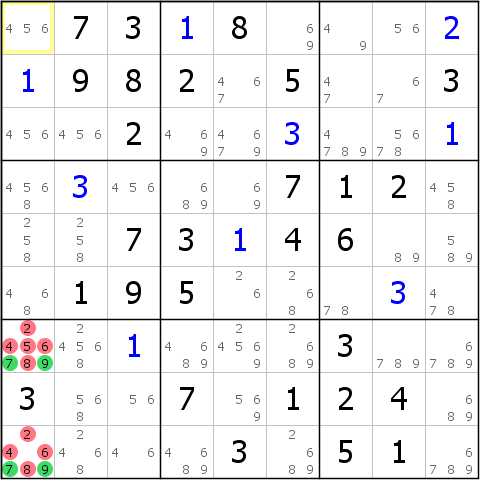
\includegraphics{./img/hidden_subset.png}
\caption{Hidden Subset - Hidden Tuple}
\end{center}
\end{figure}

\noindent In \textbf{Abbildung 2.9} betrachten wir den Block 7 und in diesem Block die Zellen z7s1 und z9s1. Nur in diesen Zellen können die Ziffern 7 und 9 in Block 7 vorkommen. Da diese zwei Ziffern nun auf die zwei Zellen verteilt werden müssen gibt, es dort keinen Platz mehr für andere Zahlen. Diese können also aus den Kandidatenlisten entfernt werden.
